\documentclass[12pt,letterpaper]{article}
\usepackage{amssymb}
\usepackage{amsmath}
\usepackage{graphicx} % Required for inserting images
\usepackage{setspace}
\usepackage[letterpaper, margin=1in]{geometry}
\usepackage[authoryear]{natbib}
\usepackage[T1]{fontenc}
\usepackage[latin9]{inputenc}
\usepackage{babel}
\usepackage{url}

\begin{document}

\doublespacing

\newcommand{\absdiv}[1]{%
 \par\addvspace{.5\baselineskip} 
  \noindent\textbf{#1} \\}

\begin{titlepage}
   \begin{center}
       \vspace*{8cm}

       \LARGE \textbf{The Dangers of Drawing Cohort Profiles From Period Data: Comment on  \citeauthor{van_raalte_dangers_2023}}
      \vspace*{3cm}
      \vfill
   \end{center}
\end{titlepage}

\clearpage

\begin{abstract}

\cite{van_raalte_dangers_2023} alert demographers to the potential dangers of calculating cohort measures from the "diagonals" of gridded age-period (AP) data. In the case of cohort fertility, however, a minor change to the estimation procedure can mitigate the trend and cohort size biases that the authors identify. With an appropriate algorithm, researchers can estimate cohort fertility indices from AP data quite well. 

\end{abstract}

\textbf{Keywords}

fertility, cohort, age-period-cohort translation, estimation methods

\clearpage


\section{Introduction}



In their first example, \cite{van_raalte_dangers_2023} address the problem estimating completed
cohort fertility levels from a 1x1 grid of AP rates $[f_{xt}]$. 
Using $\phi_{xc}$ to denote the fertility rate at integer age $x$ of the cohort
born in calendar year $c$  (an age-cohort rate
that applies to a parallelogram on the Lexis diagram), the true value
of a cohort's completed fertility at exact age 40 is 
\begin{equation}
\Phi_{c}=\sum_{x=12}^{39}\phi_{xc}\label{eq:Phi-defn}
\end{equation}
They investigate the consequences of approximating $\Phi_{c}$ by adding AP
rates from the Human Fertility Database (HFD, \citeyear{HFD2023}) over the ``diagonal'' of the Lexis grid. That is, for the cohort
born in year $c$ they calculate
\begin{equation}
F_{c}=\sum_{x=12}^{39}f_{x,c+x},\label{eq:Fc-defn}
\end{equation}
which I will call the \textit{AP
estimator}. They compare $F_{1935}\ldots F_{1982}$ to the Japanese cohort values published by the HFD. For
this example they show that proportional errors $\left(\tfrac{F_{c}-\Phi_{c}}{\Phi_{c}}\right)$
range from -2.1\% to +4.1\%, that $F_c$ systematically overestimates cohort fertility when $\Phi_{c}$ is decreasing from one cohort to the next (and underestimates when $\Phi_c$ is increasing), and that the errors
can be magnified by size differences between adjacent birth cohorts. 

In this comment I make two points about their cautionary fertility example:
\begin{itemize}
\item Raw HFD input data for Japan is in age-period format. So target
$\Phi_{c}$ values for Japan were \emph{also} estimated from a grid of Lexis
squares and $[f_{xt}]$ values, but with the multistep procedure described in the HFD Methods Protocol \citeyearpar{HFD2023}. Errors in their example measure
failure to match another algorithm, rather than failure to match true
cohort values.
\item There is a simple variant of  the AP estimator that has a stronger
demographic rationale and approximates the HFD algorithm better. This alternative procedure also has less bias  and smaller errors when tested against true 
$\Phi_{c}$ values calculated from Lexis triangle data.

\end{itemize}

As a consequence, estimating cohort fertility from age-period data
is less dangerous than implied in \cite{van_raalte_dangers_2023}'s cautionary note. 

\section{Alternative AP Diagonalization}

Formula (\ref{eq:Fc-defn}) looks reasonable, because it is a straightforward
discretization of the integral formula for cohort fertility 
on a Lexis rate surface $f(x,t)$ with continuous ages and times.
Comparing (\ref{eq:Phi-defn}) and (\ref{eq:Fc-defn}), we see that the AP estimator simply plugs in $f_{x,c+x}$ to approximate the cohort-age rate $\phi_{xc}$. 
However,  with discrete 1x1 AP squares a cohort passes through a single-year age interval over two calendar years, not one.  

Figure \ref{fig:Lexis-2-sq} illustrates with an example. The fertility rate of 1980-born women between exact ages 20 and 21 depends on births and exposure from (parts of) two AP cells: [20,2000] and [20,2001]. The AP estimate $F_{1980}$ calculated from (\ref{eq:Fc-defn}) includes data from only the first of the two relevant calendar years. This causes the backward-looking temporal bias noted by the authors. 

Intuitively, it seems that including data from both of the AP squares in the figure would produce a better approximation to the cohort-age rate. That intuition is correct.
Generalizing the specific example in Figure \ref{fig:Lexis-2-sq}, the true fertility rate at age $x$ for cohort $c$ is the ratio of births to exposure over Lexis triangles $L_{x,c+x}$ and $U_{x,c+x+1}$. Call the births in those triangles $B_L$ and $B_U$, respectively, and call the corresponding exposures $N_L$ and $N_U$. The true age-cohort rate is then

\begin{equation}
    \phi_{xc} = \frac{B_L + B_U}{N_L + N_U}
\end{equation}

The HFD and Human Mortality Database \citeyearpar{HMD2023} Methods Protocols describe careful procedures for allocating the births and exposure observed in AP cells to the underlying Lexis triangles. But there is a simple approximation to those procedures yields good estimates of cohort rates and completed fertility -- namely, assume that half of births and half of exposure in each of the two relevant AP cells belong to the cohort of interest. In that case 
\begin{equation}
    \phi_{xc} \approx \: \tfrac{1}{2}\, f_{x,c+x} \:+\: \tfrac{1}{2}\, f_{x,c+x+1}
\end{equation}
and we can construct an \textit{AP2 estimator} for completed cohort ferility by summing over ages:
\begin{equation}
\label{eq:F-tilde-defn}
    \tilde{F}_c \:= \tfrac{1}{2}\, F_c \:+\: \tfrac{1}{2}\, F_{c+1}    
\end{equation}
$\tilde{F}_c$ will not exactly equal $\Phi_c$, for several reasons (such as changing fertility rates within one-year age intervals and cohort size differences)
but it will typically be a very good approximation. Most importantly, it is not as vulnerable to temporal bias as the AP estimator $F_c$, because it is centered on the age-cohort parallelograms of interest. 


\section{Empirical Comparisons}

Figure \ref{fig:JPN vs France} compares the AP estimator from Eq. (\ref{eq:Fc-defn}) to the AP2 estimator from Eq. (\ref{eq:F-tilde-defn}). The top left panel reproduces the cautionary Japanese example in the research note \cite[Fig. 2]{van_raalte_dangers_2023} and adds the AP2 estimates as red dots connected by line segments. 

The temporal centering of the AP2 estimator greatly reduces the bias that concerned the authors. Over the 1955--1970 cohorts, for example, the AP2 estimator does not have a notable positive bias, and comes much closer than the AP estimator to matching the HFD estimates. Similarly, the AP2 estimator avoides the AP underestimates for the cohorts born after 1975. As a bonus, the errors associated with the unusually small 1966 "Fire Horse" cohort are much smaller with the temporally-centered AP2 estimates. 

The top right panel of Figure \ref{fig:JPN vs France} shows the cumulative distribution of differences between the HFD estimates of Japanese cohort fertility and the two alternatives. Large errors are much less common with the AP2 procedure, and the mean error for the AP2 estimator is close to zero (+0.1\%). 

The bottom panels of Figure \ref{fig:JPN vs France} show the equivalent results for France, a country for which the raw HFD data includes year of mother's birth. For French females cohort fertility rates are observed rather than estimated. Thus in the bottom panels we compare AP and AP2 estimates to the true cohort completed fertility levels. Results are very similar to those for Japan: the AP2 estimates do not have the temporal bias of the AP estimates when there are strong trends across cohorts, they are typically smaller than AP errors in absolute value, and the mean AP2 error is very close to zero (+0.2\%). 


\section{Conclusion}

\cite{van_raalte_dangers_2023}'s research note demonstrates that treating AP diagonal estimates as if they were true cohort measures can be problematic. It is important to consider the dangers of this procedure carefully. In the specific context of cohort fertility, however, the dangers are not as large as their research note suggests. Temporally centering the estimates by averaging two "diagonals" eliminates most of the bias problems that they highlight, and greatly mitigates the cohort-size effects. In cases like Japan the centered estimates match the HFD cohort allocation procedure very well. In cases like France they match the actual cohort data very well. With proper caution, demographers can safely "diagonalize" AP fertility rates to learn about cohorts.

\clearpage

\bibliographystyle{apalike2}
\bibliography{references}
\clearpage

\begin{figure}
    \centering
    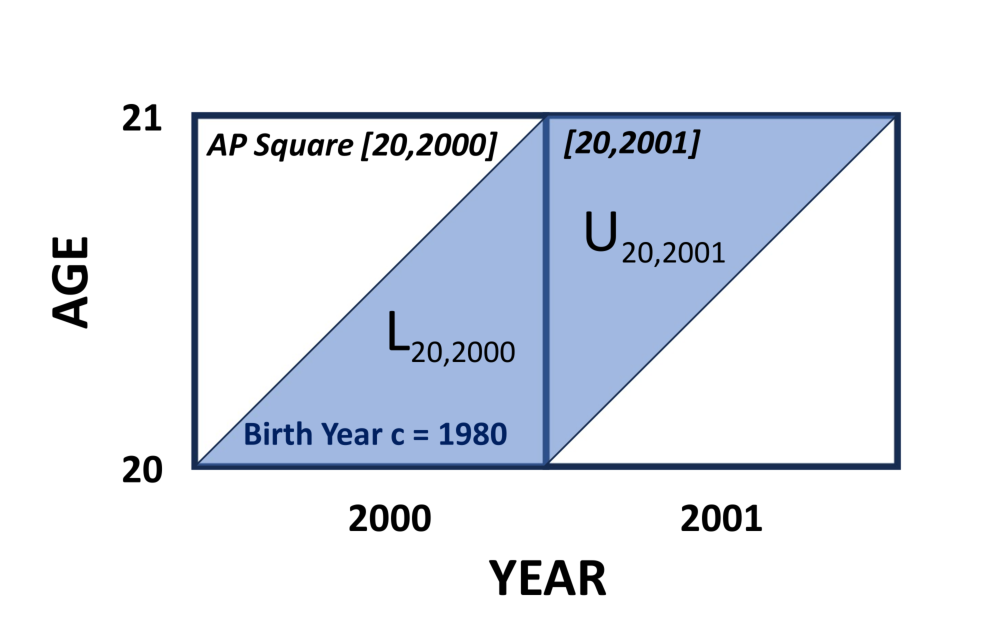
\includegraphics[width=0.6\textwidth]{Plots/2-Lexis-squares-1980-cohort.pdf}
    \caption{Lexis age-period squares, age-period-cohort triangles, and age-cohort parallelogram for the 1980 birth cohort at integer age 20. The cohort fertility rate $\phi_{20,1980}$ is the ratio of  births to exposure over triangles $L$ and $U$.}
    \label{fig:Lexis-2-sq}
\end{figure}

\clearpage

\begin{figure}
    \centering
    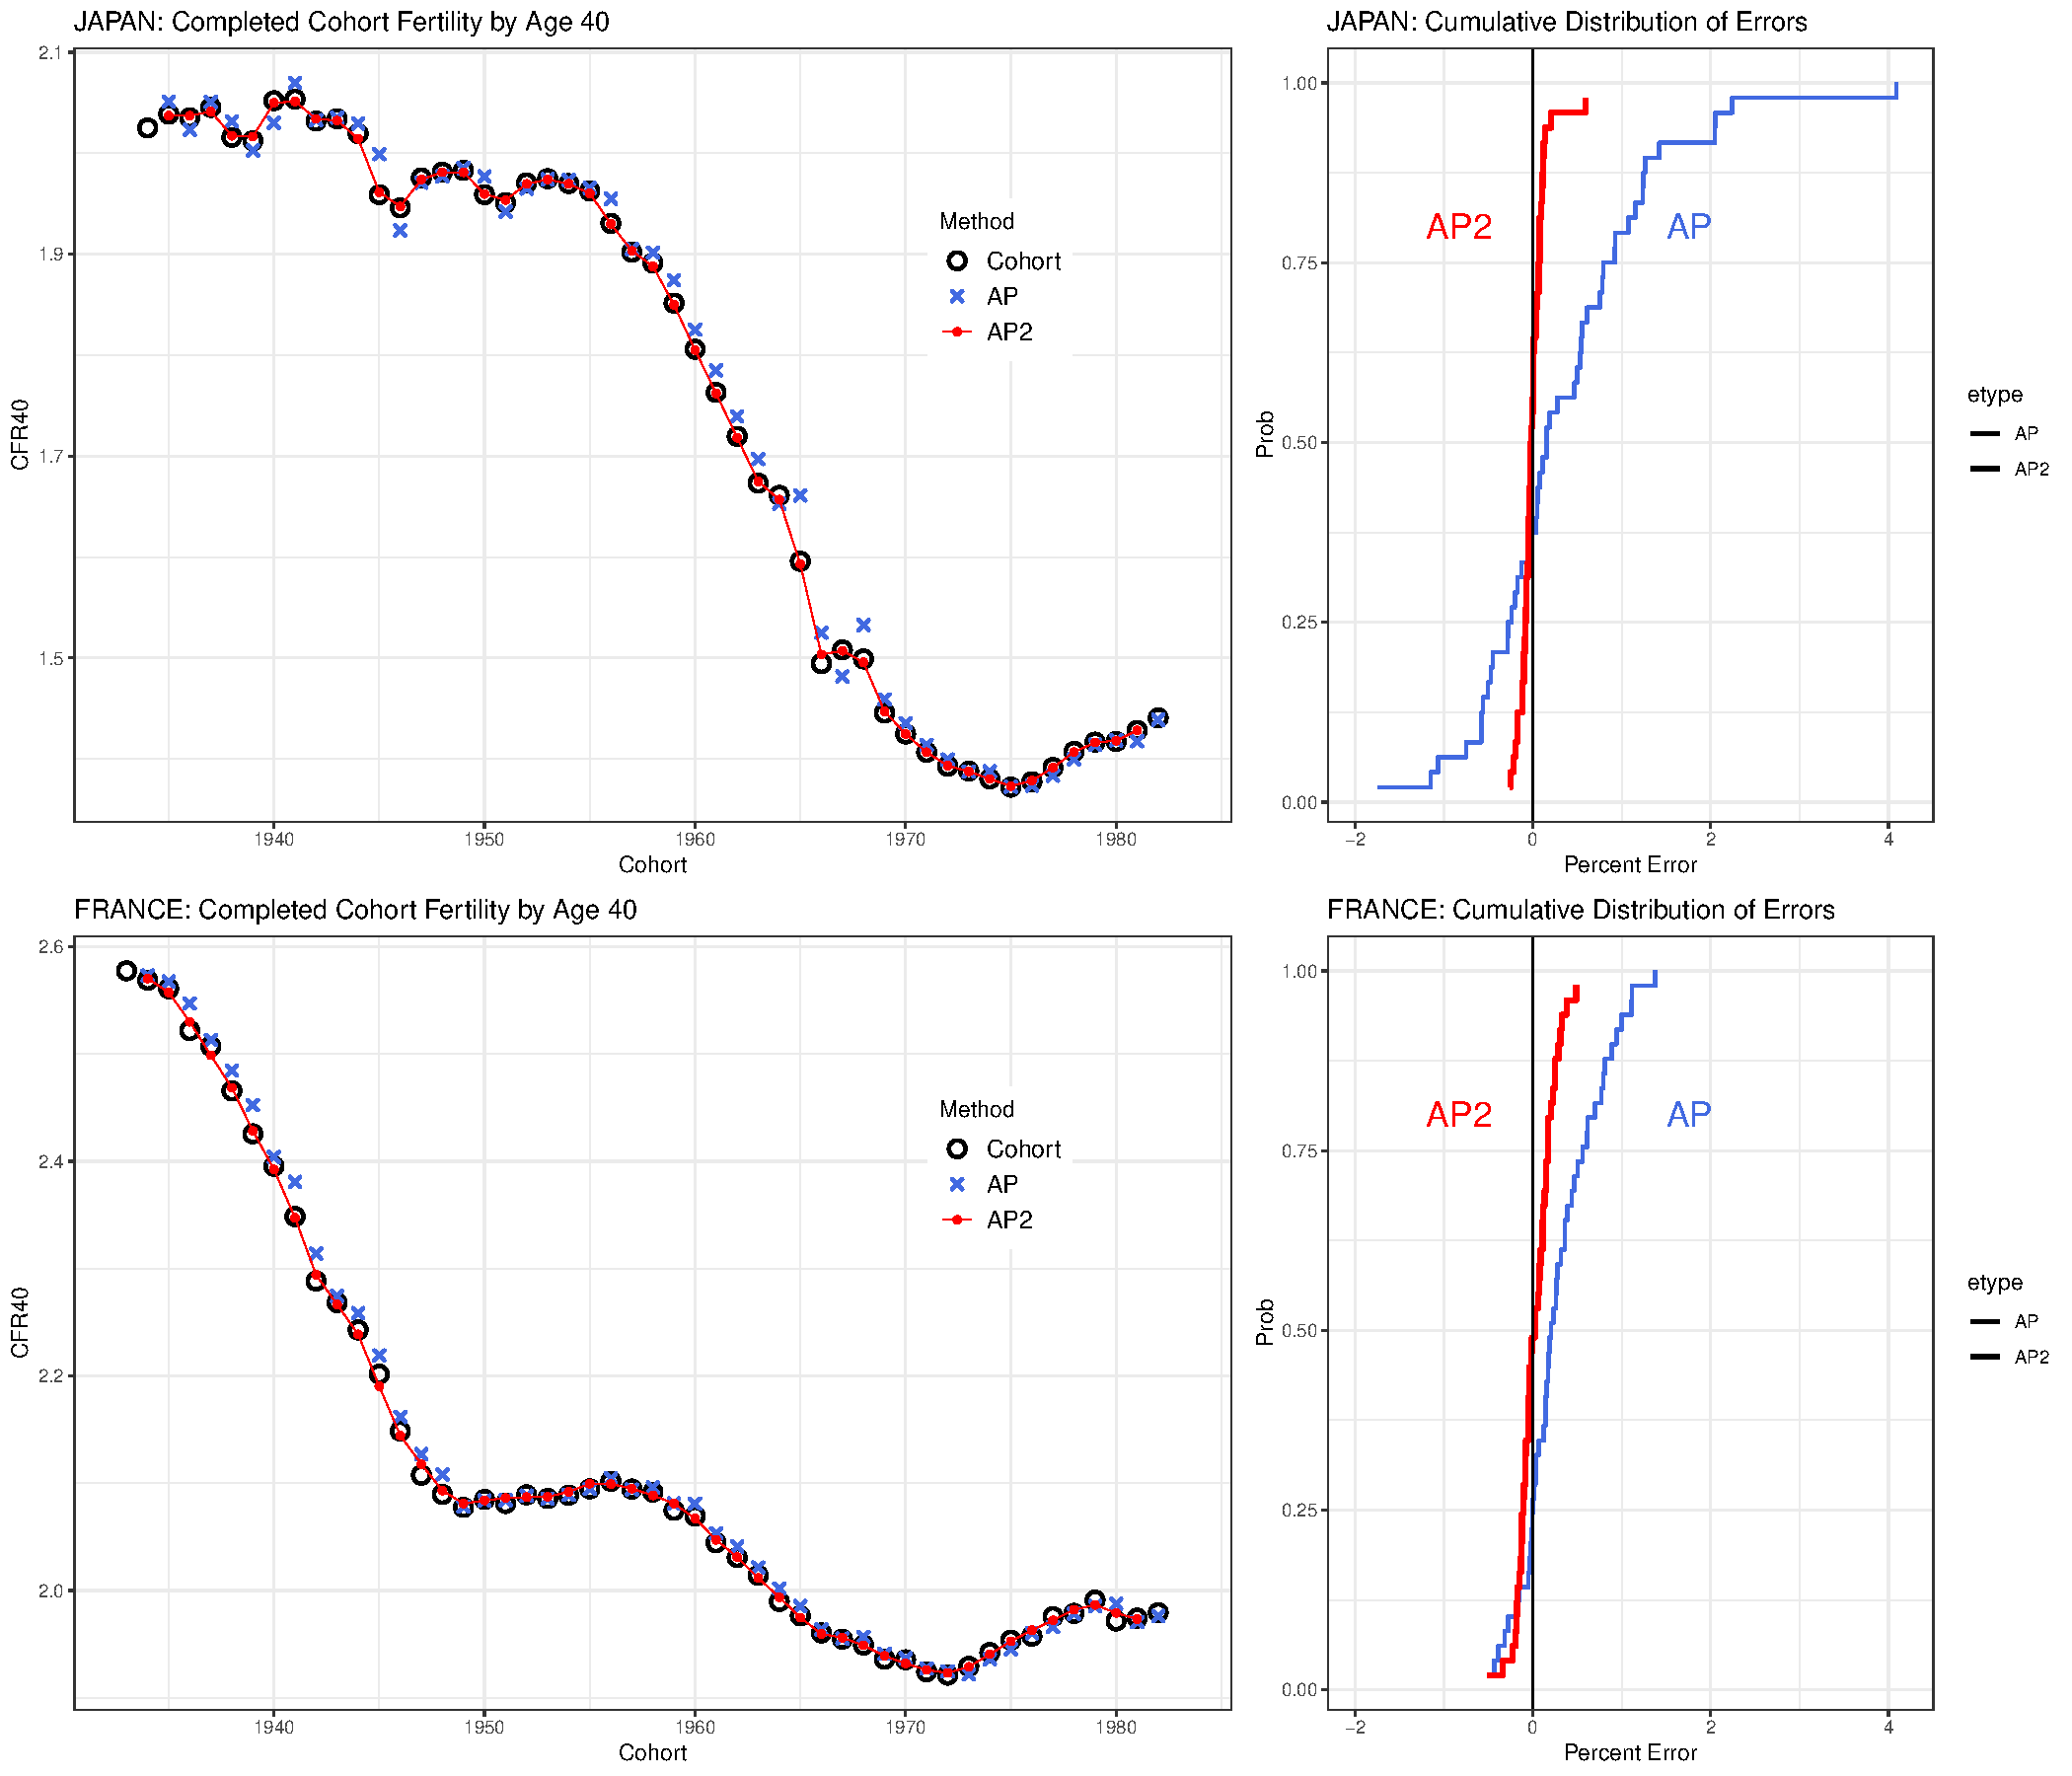
\includegraphics[width=1.0\textwidth]{Plots/2x2-summary.pdf}
    \caption{HFD cohort values and AP approximations for Japan and France. Left panels show levels of completed fertility cohort fertility published by the HFD (circles), AP estimates from Eq. (\ref{eq:Fc-defn}) using a single diagonal (blue crosses), and AP2 estimates from Eq (\ref{eq:F-tilde-defn}) that use two diagonals (solid red dots with connecting lines). Right panels show the cumulative distributions of AP and AP2 errors across birth cohorts.}
    \label{fig:JPN vs France}
\end{figure}

\end{document}
